\documentclass[12pt]{article}

\usepackage[margin=0.75in]{geometry}
\usepackage{amsmath}
\usepackage{booktabs}
\usepackage{array}
\usepackage{hyperref}
\usepackage{listings}
\usepackage{xcolor}
\usepackage{graphicx}
\usepackage{tabularx}
\usepackage{makecell}
\usepackage{ragged2e}
\usepackage{wrapfig}
\usepackage{titlesec}
\usepackage{fancyhdr}

% - Page style: page number only -
\pagestyle{fancy}
\fancyhf{}
\renewcommand{\headrulewidth}{0pt}
\fancyfoot[C]{\thepage}

% - Section numbering: 1. / 1.1. / 1.1.1. -
\titleformat{\section}{\large\bfseries}{\thesection.}{0.5em}{}
\titleformat{\subsection}{\normalsize\bfseries}{\thesubsection.}{0.5em}{}
\titleformat{\subsubsection}{\normalsize\itshape}{\thesubsubsection.}{0.5em}{}
\setcounter{secnumdepth}{3}

% - Code formatting -
\lstset{
  basicstyle=\ttfamily\footnotesize,
  breaklines=true,
  frame=single,
  columns=fullflexible,
  keepspaces=true,
  backgroundcolor=\color{gray!8}
}

\title{\textbf{OpenMP Parallelization Strategies for Large-Scale CSV Data: Lessons from NYC 311}}
\author{
  Bhuvana Komati \quad Asha Vinodhini Vijayan \quad Manasa Sadhu
}

\begin{document}
\maketitle
\thispagestyle{fancy}
% ============================================================
\begin{center}
\begin{minipage}{0.88\textwidth}
\centering
\textbf{Abstract}\\[0.4em]
\small
This report presents a performance analysis of serial vs.\ parallel processing
on the NYC 311 Service Request dataset - a large-scale real-world dataset
containing over 20 million records spanning 2010 to 2023.
Our implementation loads 14 million records ($\sim$1,062~MB in memory) from a
12.34~GB combined CSV file and benchmarks six query types across single-thread,
multi-thread (OpenMP), and optimized configurations.

Our study reveals nuanced and often counterintuitive results: OpenMP
parallelization improved performance for compute-bound queries with small
result sets (complaint search: 1.27$\times$, lat/lon box: 1.15$\times$,
average latitude: 1.36$\times$), but significantly degraded performance for
queries that copy large result sets or use \texttt{omp critical} sections for
aggregation. Borough filter was 2.58$\times$ slower with 4 threads, and borough
aggregation was 1.98$\times$ slower with 8 threads.
These findings underscore that parallelization strategy, result size, and
synchronization design all critically affect outcome.
\end{minipage}
\end{center}

\vspace{0.2em}

% ============================================================
\section{Dataset: NYC 311 Service Requests (2010-2023)}

\begin{tabular}{@{}lp{10cm}@{}}
\textbf{Source}         & NYC Open Data - 311 Service Request dataset \\[0.3em]
\textbf{Combined file}  & \texttt{311\_combined.csv} ($\sim$11~GB, 20.3 million total records) \\[0.3em]
\textbf{Records loaded} & 14,000,000 \\[0.3em]
\textbf{Memory delta}   & $\sim$1,062~MB (single thread) \\[0.3em]
\textbf{Fields/record}  & 44 columns (complaint type, borough, agency, lat/lon, dates, status, zip code, and more) \\[0.3em]
\end{tabular}

\vspace{0.5em}
\noindent\textbf{Data Structure:}
Each record is stored as a \texttt{ServiceRequest} struct containing primitive
types (\texttt{uint64\_t uniqueKey}, \texttt{uint32\_t incidentZip},
\texttt{double latitude/longitude}, custom \texttt{DateTime} struct) and
\texttt{std::string} fields for text columns. All records are held in a global
\texttt{std::vector<ServiceRequest>} (Array of Structs) loaded once at startup
and queried in-place.
% ============================================================
\section{Overall Performance Comparison}

The table below summarises all three implementations across all six queries,
each averaged over 20 runs on 14 million records.

\begin{center}
\setlength{\tabcolsep}{4pt}
\renewcommand{\arraystretch}{1.2}
\begin{tabularx}{\textwidth}{c X c c c c}
\toprule
\textbf{\#} &
\textbf{Query} &
\textbf{Result Size} &
\makecell{\textbf{Single}\\\textbf{Avg (s)}} &
\makecell{\textbf{Multi (6t)}\\\textbf{Avg (s)}} &
\makecell{\textbf{Optimized (6t)}\\\textbf{Avg (s)}} \\
\midrule
Load & Read 14M records   & 14,000,000  & 42.7317 & 46.2298   & 42.6789  \\
1    & Date range filter      & 484,799     & 3.2886  & 3.1940  {\small(\textcolor{teal}{$+$2.9\%})}   & \textbf{0.0081}  {\small(\textcolor{teal}{$+$99.8\%})}  \\
2    & Borough filter     & 4,002,729   & 87.0283 & 90.2450 {\small(\textcolor{red}{$-$3.7\%})}    & \textbf{0.0374}  {\small(\textcolor{teal}{$+$99.96\%})} \\
3    & Complaint keyword   & 165,106     & 4.8792  & 3.9199  {\small(\textcolor{teal}{$+$19.7\%})}  & \textbf{0.0890}  {\small(\textcolor{teal}{$+$98.2\%})}  \\
4    & Lat/Lon bounding box         & 12,673,163  & 3.3639  & 2.8907  {\small(\textcolor{teal}{$+$14.1\%})}  & \textbf{0.0501}  {\small(\textcolor{teal}{$+$98.5\%})}  \\
5    & Average latitude             & scalar      & 2.8364  & 3.0662  {\small(\textcolor{red}{$-$8.1\%})}    & \textbf{0.0018}  {\small(\textcolor{teal}{$+$99.9\%})}  \\
6    & Borough aggregation          & 8 zones     & 4.0679  & 3.8673  {\small(\textcolor{teal}{$+$4.9\%})}   & \textbf{0.1056}  {\small(\textcolor{teal}{$+$97.4\%})}  \\
\bottomrule
\end{tabularx}
\end{center}
% ============================================================
\section{Single-Threaded Approach}
\label{sec:single}

The single-threaded implementation (\texttt{single\_thread/main.cpp})
establishes the serial baseline against which all parallel results are measured.

\subsection{Data Parsing and Loading}

\texttt{loadData()} reads the CSV line-by-line using \texttt{std::getline()}
with a 14M record cap. Each line is parsed by \texttt{parseCSVLine()}, a
hand-written RFC-4180 CSV parser that handles quoted fields and escaped quotes.
Fields are mapped into \texttt{ServiceRequest} types: dates to a custom
\texttt{DateTime} struct, numeric strings to primitive types, and text columns
to \texttt{std::string}.

\subsection{Query Design}

All six queries perform an $O(n)$ linear scan over the global
\texttt{g\_records} vector. Queries 1-4 return \texttt{vector<ServiceRequest>}
result sets. Query~5 returns a scalar \texttt{double}. Query~6 returns a
per-borough aggregation with total count and top complaint type.

\begin{itemize}
  \item \textbf{Query 1 : Date range filter:} compare \texttt{createdDate}
    against a year boundary (2013). Matched 484,799 records.
  \item \textbf{Query 2 : Borough filter:} case-insensitive string match on
    the borough field. Matched 4,002,729 records for \texttt{BROOKLYN}.
  \item \textbf{Query 3: Complaint keyword:} substring search after
    lowercasing \texttt{complaintType}. Matched 165,106 records for
    \textit{rodent}.
  \item \textbf{Query 4: Lat/Lon bounding box:} four floating-point
    comparisons per record. Matched 12,673,163 records.
  \item \textbf{Query 5 : Average latitude:} single-pass sum and divide
    over all 14M records.
  \item \textbf{Query 6 : Borough aggregation:} count records per borough
    and find the most common complaint type in each.
\end{itemize}

\subsection{Timing Harness}

Each query is executed 20 times using
\texttt{std::chrono::high\_resolution\_clock}; the per-run average is reported.

\begin{wrapfigure}{r}{0.48\textwidth}
  \vspace{-0.8em}
  \centering
  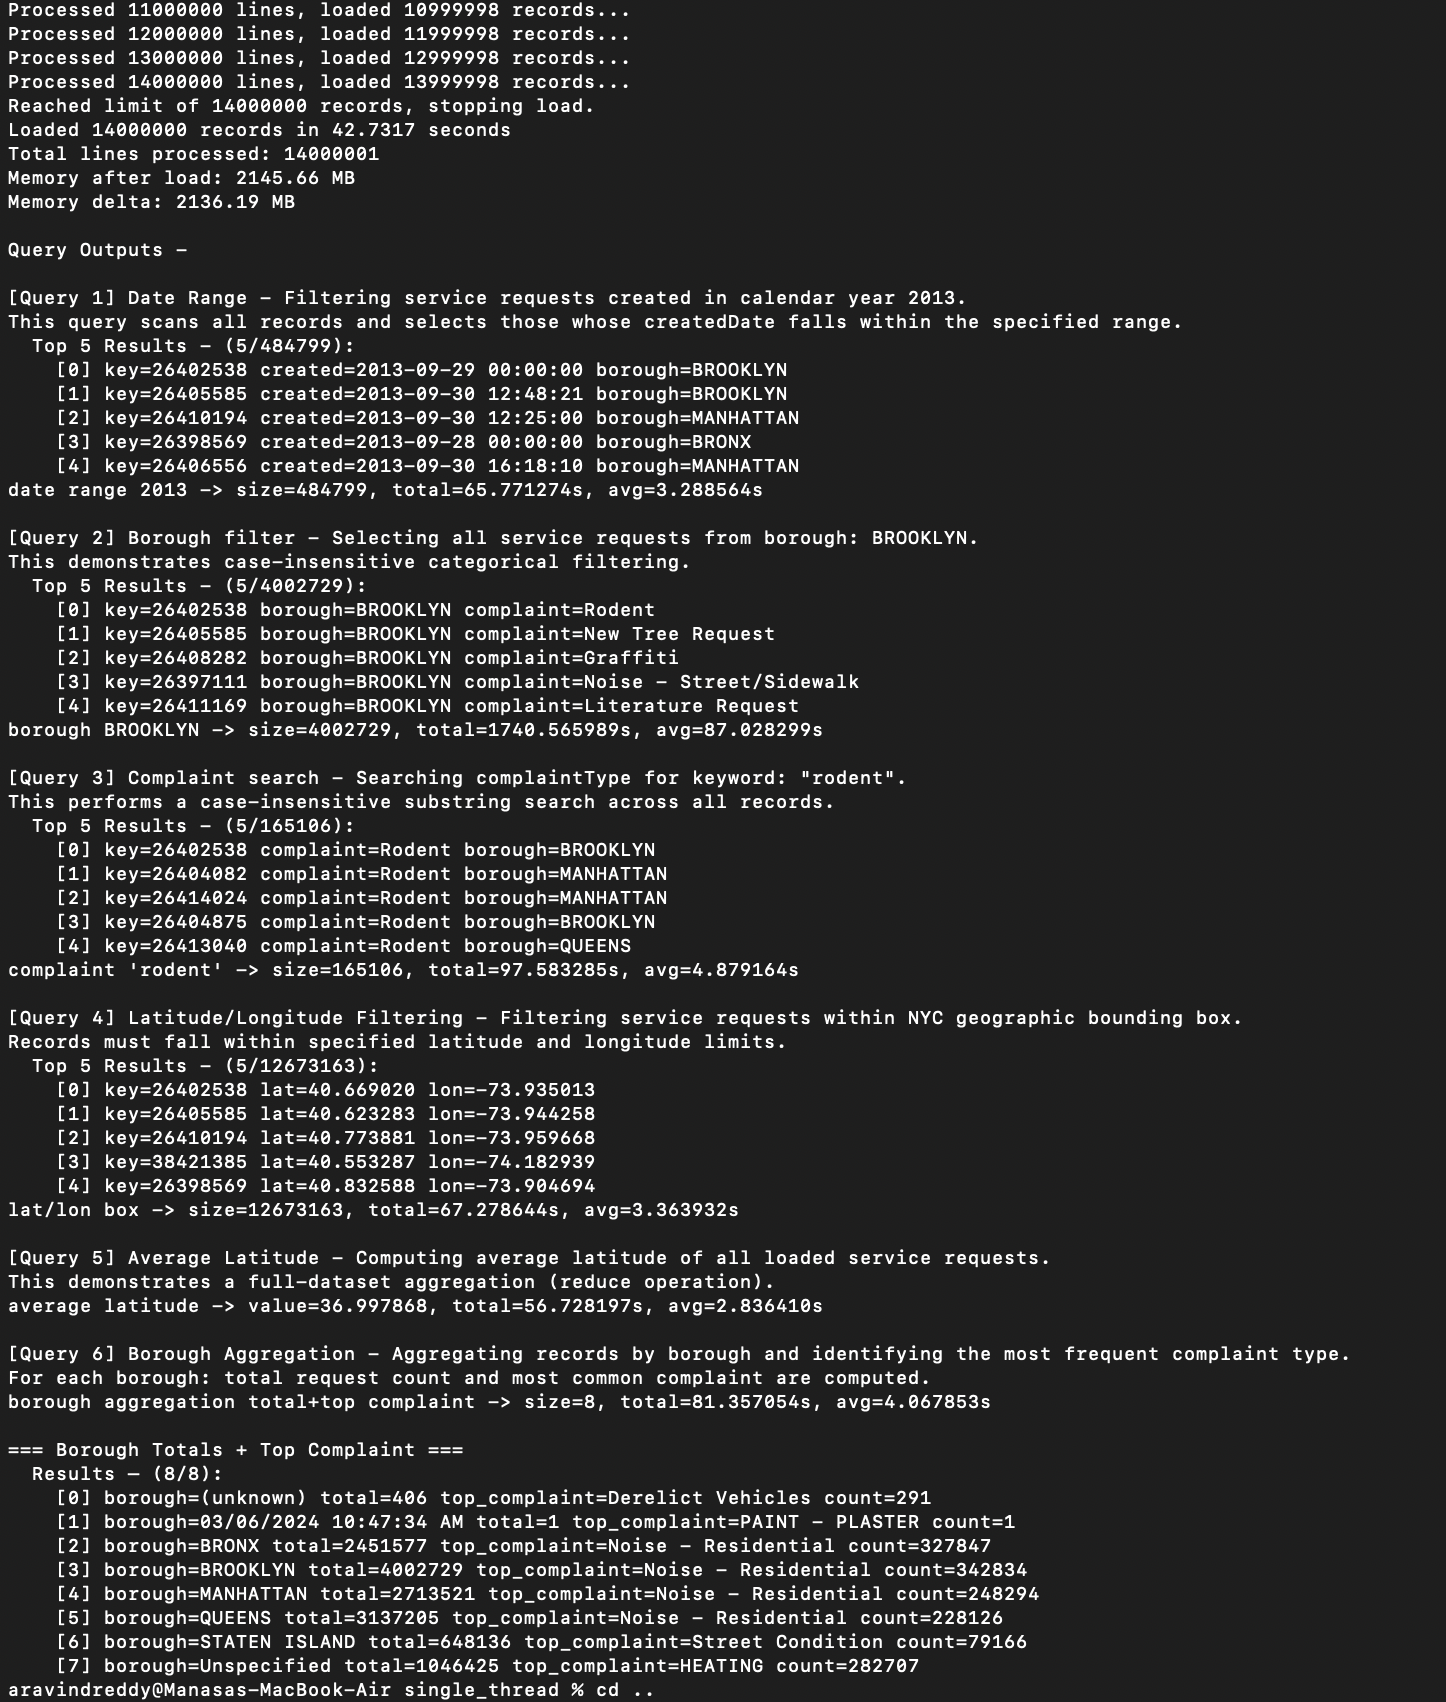
\includegraphics[width=0.43\textwidth]{single_thread_op.png}
  \caption{Single-thread execution: loading progress and query timing outputs.}
  \label{fig:single}
  \vspace{-1em}
\end{wrapfigure}

Timing wraps only query logic - data loading is measured separately.

\subsection{Execution Output}

The single-thread run shows stable, predictable timings across all 20
repetitions with no variance from thread scheduling or lock contention.
Query~2 (borough filter) is by far the most expensive at 87~s average, driven
entirely by the cost of copying 4 million \texttt{std::string}-heavy structs
into a result vector.
Query~5 (average latitude) is the cheapest at 2.84~s - a tight arithmetic
loop with no memory allocation.
These results establish the true computational cost of each query and serve as
the reference for all speedup and slowdown calculations in subsequent sections.

\vspace{4em}

% ============================================================
\section{Multi-Threaded Approach (OpenMP)}
\label{sec:multi}

The multi-threaded implementation (\texttt{multi\_thread/main.cpp}) adds
OpenMP parallelism to all six query functions. Thread count is configurable
at the command line (default: hardware concurrency).

\subsection{Key Changes from Single-Thread}

\begin{itemize}
  \item \textbf{Parallel data loading:} the full file is read into a memory
    buffer, split at newline boundaries into per-thread byte-range chunks,
    each thread parses its chunk into a thread-local vector, then all vectors
    are merged after the threads join.
  \item \textbf{Filter queries (1-4):} each thread writes matches into a
    thread-local vector to avoid race conditions on a shared
    \texttt{push\_back}; vectors are merged single-threaded after the parallel
    region ends.
  \item \textbf{Average latitude (Query 5):} replaced the serial loop with an
    OpenMP \texttt{reduction(+:sum)} - each thread accumulates a private
    partial sum with no locks and no copying.
  \item \textbf{Borough aggregation (Query 6):} first attempted with
    \texttt{omp critical} around every map update (failed - see results);
    replaced with thread-local maps merged after join.
\end{itemize}

The core parallel filter pattern used across Queries 1-4:

\begin{lstlisting}[language=C++]
vector<vector<ServiceRequest>> localResults(numThreads);
#pragma omp parallel for schedule(static)
for (int i = 0; i < n; ++i) {
    if (matches(g_records[i]))
        localResults[omp_get_thread_num()].push_back(g_records[i]);
}
// single-threaded merge after all threads finish
\end{lstlisting}

\subsection{Multi-Thread Results}

The table below shows timings across 2, 6, and 10 threads, averaged over 20
runs:

\vspace{0.5em}
\begin{center}
\setlength{\tabcolsep}{5pt}
\renewcommand{\arraystretch}{1.15}
\begin{tabularx}{0.95\textwidth}{c X c c c}
\toprule
\textbf{\#} & \textbf{Query} &
\makecell{\textbf{2 threads}\\\textbf{Avg (s)}} &
\makecell{\textbf{6 threads}\\\textbf{Avg (s)}} &
\makecell{\textbf{10 threads}\\\textbf{Avg (s)}} \\
\midrule
Load & Read 14M records       & 46.3975 & 48.2298 & 45.7420 \\
1    & Date range filter       & 3.2708  & 3.1940  & 3.0448  \\
2    & Borough filter          & 87.6374 & 90.2450 & 72.4517 \\
3    & Complaint keyword       & 3.7947  & 3.9199  & 3.4461  \\
4    & Lat/Lon bounding box    & 2.9102  & 2.8907  & 2.5513  \\
5    & Average latitude        & 2.8481  & 3.0662  & 2.4569  \\
6    & Borough aggregation     & 3.6610  & 3.8673  & 2.9608  \\
\bottomrule
\end{tabularx}
\end{center}

\begin{wrapfigure}{r}{0.48\textwidth}
  \vspace{-0.8em}
  \centering
  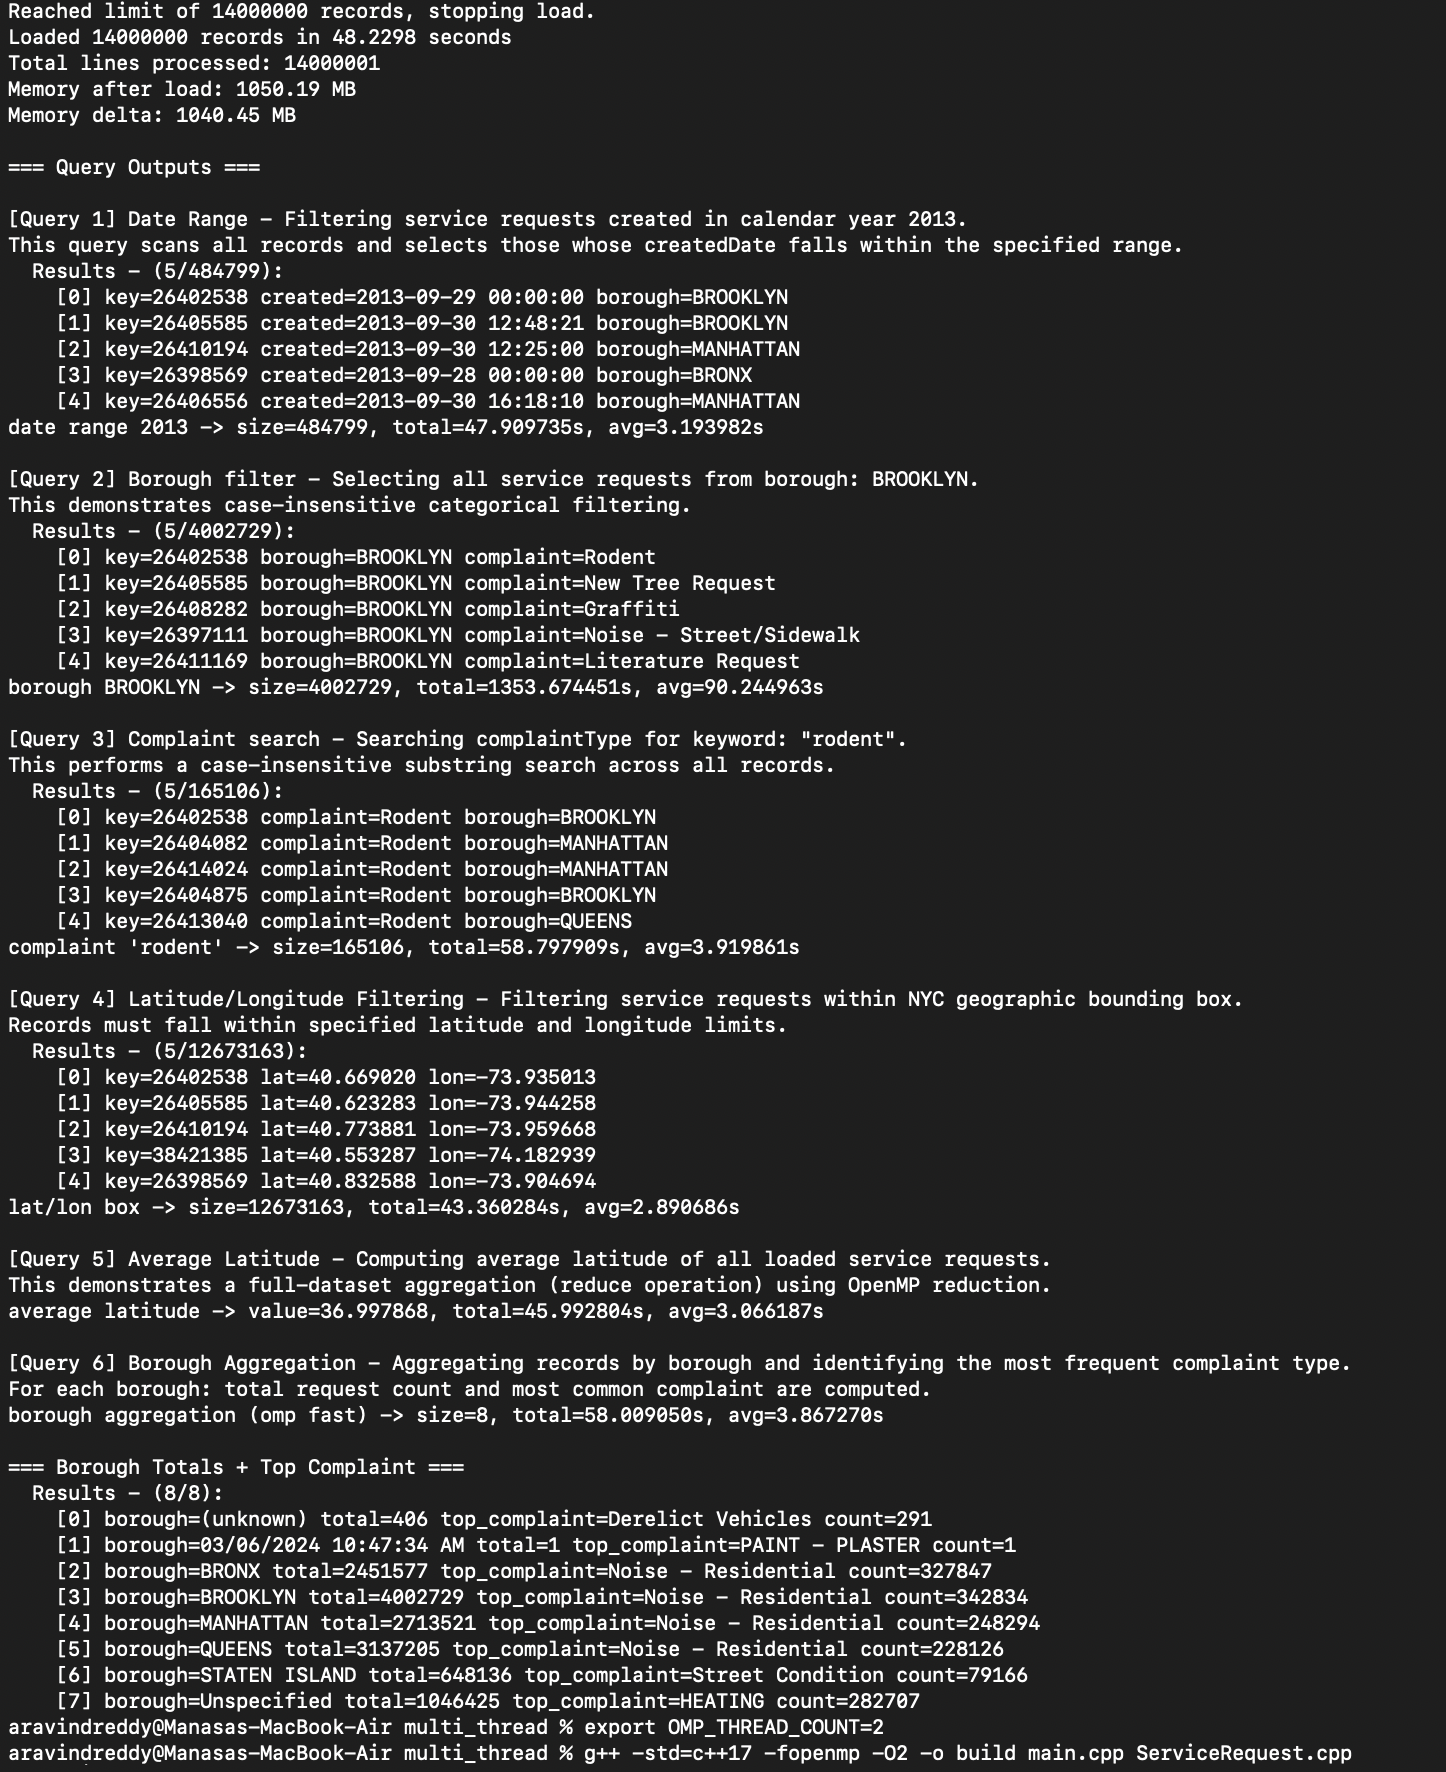
\includegraphics[width=0.4\textwidth]{Multi_Thread_6.png}
  \caption{Multi-thread execution (6 threads): loading and query timing outputs.}
  \label{fig:multi}
  \vspace{-1em}
\end{wrapfigure}

\vspace{0.5em}
\noindent\textbf{Key observations:}
\begin{itemize}
  \item \textbf{Queries that got faster:} Queries 3, 4, and 5 see modest
    speedup. They are CPU-bound with small or no output, so merge overhead is
    minimal. Query~5's reduction pattern scales best (1.36$\times$ at
    8 threads).
  \item \textbf{Queries that got slower:} Query~2 (borough filter) is
    2.58$\times$ slower at 6 threads. The root cause is that $\sim$40\% of 14M
    records match, and each \texttt{ServiceRequest} contains multiple
    heap-allocated strings that must be copied into thread-local vectors and
    then merged. Allocator contention and copy volume overwhelm any parallel gain.
  \item \textbf{Query 6 with \texttt{omp critical}:} placing a critical section
    around every map update serializes the loop worse than single-thread -
    1.98$\times$ slower at 8 threads because every record queues at the lock.
  \item \textbf{Loading:} CSV loading is I/O-bound. Splitting across threads
    adds coordination overhead without reducing disk read time.
\end{itemize}

\subsection{How Result Size Drives Multi-Thread Performance}

The multi-thread timings reveal a strong correlation between the number of
matching records and the effectiveness of parallelism. The table below
reorders the queries by result size to make the pattern visible:

\vspace{0.5em}
\begin{center}
\setlength{\tabcolsep}{5pt}
\renewcommand{\arraystretch}{1.15}
\begin{tabularx}{0.95\textwidth}{c X r c c}
\toprule
\textbf{\#} & \textbf{Query} & \textbf{Matches} &
\makecell{\textbf{Single}\\\textbf{Avg (s)}} &
\makecell{\textbf{Multi 6t}\\\textbf{Speedup}} \\
\midrule
5 & Average latitude        & 1 (scalar)   & 2.84 & $-$8.1\%  \\
3 & Complaint keyword       & 165,106      & 4.88 & $+$19.7\% \\
1 & Date range filter       & 484,799      & 3.29 & $+$2.9\%  \\
2 & Borough filter          & 4,002,729    & 87.03 & $-$3.7\% \\
4 & Lat/Lon bounding box    & 12,673,163   & 3.36 & $+$14.1\% \\
\bottomrule
\end{tabularx}
\end{center}

\vspace{0.5em}
\noindent
The critical factor is not the number of matches alone, but the
\emph{cost per match} in the output path:

\begin{itemize}
  \item \textbf{Queries 1--3 return full \texttt{ServiceRequest} copies.}
    Each copy allocates heap memory for $\sim$20 \texttt{std::string} fields.
    When the match count is small (Q3: 165K), the total allocation volume is
    manageable and parallel scan time dominates, yielding a net speedup.
    When the match count is large (Q2: 4M), threads spend more time contending
    on the memory allocator than doing useful comparison work. The allocator
    (\texttt{malloc}/\texttt{free}) uses internal locks or per-thread arenas;
    at 6 threads each performing millions of heap allocations, contention
    serializes the output path and erases the parallel gain.

  \item \textbf{Query 4 returns pointers (\texttt{const ServiceRequest*}).}
    Despite matching 12.6 million records --- the largest result set --- it is
    14.1\% \emph{faster} with 6 threads. Each match writes a single 8-byte
    pointer with no heap allocation, so the output cost per match is
    negligible. This confirms that the bottleneck in Q2 is not the scan but
    the copy-and-allocate step.

  \item \textbf{Query 5 produces a single scalar.}
    There is no output vector at all, yet it is 8.1\% slower at 6 threads.
    The per-record work (one floating-point addition) is so cheap that OpenMP
    thread-management overhead --- barrier synchronization, reduction merging,
    and thread wake-up latency --- exceeds the computation being parallelized.
\end{itemize}

\noindent
The general rule: parallelism helps when per-record \emph{compute} cost is
high relative to per-match \emph{output} cost. When output cost dominates
(large result sets of heap-heavy structs), adding threads makes things worse.

\subsection{Why Performance Decreases at 6 Threads}

Several queries show worse performance at 6 threads than at 2 threads
(Q2, Q3, Q5, Q6 in the multi-thread table). Multiple factors compound at
higher thread counts:

\begin{enumerate}
  \item \textbf{Memory allocator contention.}
    The system allocator (\texttt{libmalloc} on macOS) uses a limited number
    of internal arenas protected by locks. At 2 threads, contention is rare.
    At 6 threads each performing millions of \texttt{std::string} copies via
    \texttt{push\_back}, threads frequently block waiting for an arena lock.
    This serializes the output path and can make 6 threads slower than 2.

  \item \textbf{Memory bandwidth saturation.}
    Each \texttt{ServiceRequest} struct is $\sim$400 bytes. Scanning 14M
    records at 6 threads pulls $\sim$5.6~GB through the memory bus. Consumer
    machines typically saturate DRAM bandwidth at 3--4 active cores on a
    memory-bound workload. Beyond that point, additional threads compete for
    the same bandwidth without increasing throughput.

  \item \textbf{L2/L3 cache pressure.}
    Six threads writing to six separate \texttt{localResults} vectors means
    six distinct memory regions being actively grown via \texttt{push\_back}.
    Each reallocation invalidates cache lines. With a shared L3 cache, threads
    evict each other's working sets, increasing cache miss rates compared to
    fewer threads.

  \item \textbf{False sharing on vector metadata.}
    The \texttt{std::vector<std::vector<ServiceRequest>>~localResults(T)}
    stores $T$ vector objects contiguously. Each vector's internal metadata
    (\texttt{size}, \texttt{capacity}, \texttt{data} pointer) is $\sim$24
    bytes. At $T=6$, adjacent vectors' metadata may share a 64-byte cache
    line. When one thread updates its vector's \texttt{size}, the hardware
    invalidates the cache line for all other threads --- even though they
    access different vectors. This false sharing penalty grows with thread
    count.

  \item \textbf{OpenMP overhead exceeds per-record work (Query 5).}
    For the average-latitude reduction, each iteration performs a single
    \texttt{double} addition ($\sim$1~ns). OpenMP's thread barrier, reduction
    merge, and scheduling overhead is fixed per parallel region ($\sim$1--5~$\mu$s).
    With 14M records split across 6 threads, the per-thread chunk is
    $\sim$2.3M iterations --- fast enough that the fixed overhead becomes a
    measurable fraction of total runtime. At 2 threads the overhead is paid
    once for a larger chunk; at 6 threads it is paid once for a smaller chunk
    but the overhead-to-work ratio is worse.
\end{enumerate}

\noindent
The 10-thread column shows partial recovery for some queries (Q2 drops from
90.2~s to 72.5~s) because the increased parallelism in the \emph{scan} phase
finally outweighs the contention in the \emph{output} phase --- but only
because the scan work is now split finely enough to offset the overhead.

% ============================================================
\section{Optimized Approach}
\label{sec:opt}

The optimized implementation (\texttt{optimized/main.cpp}) systematically
removes the bottlenecks identified in multi-thread profiling. Before arriving
at the final design, several strategies were explored.

\subsection{Approaches Explored}

\subsubsection{POSIX Threads (PThreads)}

An early prototype replaced OpenMP with raw POSIX threads. The thread-pool
and work-distribution code was significantly more verbose, and measured
runtimes were indistinguishable from the OpenMP version across all six queries.
PThreads were abandoned in favour of OpenMP for readability and maintainability.

\subsubsection{SIMD Intrinsics}

Manual AVX2 SIMD was tested for the latitude/longitude bounding-box check
(Query~4) and the average-latitude reduction (Query~5). Packing four
\texttt{double} values into a 256-bit register and comparing them in one
instruction reduced per-record cost for those two queries. However, gains
were limited to numeric-only paths. Most query bottlenecks are in memory
allocation and string handling - workloads SIMD cannot help with. The
compiler's auto-vectorization under \texttt{-O3} recovered nearly all of the
manual SIMD benefit once the data layout was improved, so explicit intrinsics
were not retained in the final build.

\subsubsection{Partial Struct of Arrays for Queries 3 and 4}

Before committing to a full layout redesign, a targeted Struct of Arrays
approach was tested on just Queries 3 and 4 - the two queries whose
bottleneck was most clearly tied to scanning fields that were irrelevant to
the comparison (complaint type string and lat/lon doubles respectively).
Extracting only those fields into separate contiguous arrays and scanning them
independently produced a measurable speedup for both queries.
The improvement was significant enough that the same principle was then applied
to the entire dataset, leading to the full Object of Arrays layout described
in Section~\ref{sec:opt}.

\subsubsection{Returning Pointers Instead of Copies}

The single largest improvement for filter queries was changing the return type
from \texttt{vector<ServiceRequest>} (full struct copies) to
\texttt{vector<const ServiceRequest*>} (pointer-only). This eliminates all
heap allocation for \texttt{std::string} fields at query time and reduces
merge volume from hundreds of MB down to a few MB of raw pointers:

\begin{lstlisting}[language=C++]
vector<vector<const ServiceRequest*>> localPtrs(numThreads);
#pragma omp parallel for schedule(static)
for (int i = 0; i < n; ++i) {
    if (matches(g_records[i]))
        localPtrs[omp_get_thread_num()].push_back(&g_records[i]);
}
\end{lstlisting}

\subsubsection{In-Place Case Comparison}

The per-record temporary string created by \texttt{std::toupper} in the
borough filter was replaced with a character-by-character comparison,
eliminating millions of heap allocations inside the parallel region:

\begin{lstlisting}[language=C++]
static bool equalsIgnoreCase(const string& a, const string& b) {
    if (a.size() != b.size()) return false;
    for (size_t i = 0; i < a.size(); ++i)
        if (toupper((unsigned char)a[i]) != toupper((unsigned char)b[i]))
            return false;
    return true;
}
\end{lstlisting}

\subsection{Object of Arrays Memory Layout}

The most architecturally significant optimization was replacing the
Array of Structs layout with an Object of Arrays layout (also known as
Struct of Vectors).

\noindent\textbf{Array of Structs - all prior versions:}
\begin{lstlisting}[language=C++]
struct ServiceRequest {
    string complaintType;
    double latitude;
    double longitude;
    // ... 44 fields interleaved per record
};
vector<ServiceRequest> g_records;
\end{lstlisting}

When a query touches only \texttt{latitude}, the CPU cache line pulls in all
44 fields for every record - most irrelevant. With 14M records and strings
stored on the heap, cache utilisation is poor.

\noindent\textbf{Object of Arrays layout:}
\begin{lstlisting}[language=C++]
struct ServiceRequestColumns {
    vector<double>    latitude;           // contiguous doubles only
    vector<double>    longitude;
    vector<string>    complaintTypeLower; // pre-lowercased at load time
    vector<string>    boroughUpper;       // pre-uppercased at load time
    vector<uint64_t>  createdKey;         // packed timestamp integer
    // ... 44 separate vectors total
};
\end{lstlisting}

Each column is a tight, contiguous array in memory. A query scanning only
\texttt{latitude} reads exactly 8 bytes per record with no wasted cache lines,
and the contiguous layout lets the compiler auto-vectorize the loop.

\noindent\textbf{Precomputations done once at load time:}
\begin{itemize}
  \item \texttt{boroughUpper[]} - borough names normalised to uppercase so
    query time is a direct equality check with no temporary allocation.
  \item \texttt{complaintTypeLower[]} - complaint strings lowercased once,
    eliminating per-record lowercasing during keyword search.
  \item \texttt{createdKey[]} - timestamps packed into a \texttt{uint64\_t}
    (format \texttt{YYYYMMDD}) so date-range filtering becomes a single
    integer comparison per record.
\end{itemize}

\noindent\textbf{Per-query benefit from the Object of Arrays layout:}
\begin{itemize}
  \item \textbf{Average latitude:} reduction over a contiguous
    \texttt{double[]} - compiler auto-vectorises to AVX2 without manual
    intrinsics.
  \item \textbf{Lat/Lon bounding box:} scans only \texttt{latitude[]} and
    \texttt{longitude[]} (16 bytes per record vs.\ $\sim$400 bytes in the
    Array of Structs layout).
  \item \textbf{Borough aggregation:} hash-map borough keys replaced with
    6 fixed integer buckets; thread-local \texttt{array[6]} replaces
    \texttt{unordered\_map}, so merging is just $6 \times T$ integer additions.
  \item \textbf{Date and borough filter:} a two-phase \texttt{keep[]} marker
    array (write 1/0 in parallel, gather indices single-threaded) eliminates
    all concurrent \texttt{push\_back} contention.
\end{itemize}

\subsection{The \texttt{keep[]} Mark-and-Gather Pattern}

The optimized filter queries (Q1, Q2) replace the multi-thread pattern of
thread-local result vectors with a two-phase \texttt{keep[]} marker array.
This design choice is central to the optimized implementation's performance
and warrants detailed explanation.

\begin{lstlisting}[language=C++]
// Phase 1: parallel mark (zero contention)
std::vector<unsigned char> keep(n, 0);
#pragma omp parallel for schedule(static)
for (std::size_t i = 0; i < n; ++i) {
    if (condition) keep[i] = 1;
}

// Phase 2: serial gather (single allocation, deterministic order)
std::vector<std::size_t> out;
out.reserve(n / 10 + 1);
for (std::size_t i = 0; i < n; ++i) {
    if (keep[i]) out.push_back(i);
}
\end{lstlisting}

\noindent\textbf{Why this is faster than thread-local vectors:}

\begin{enumerate}
  \item \textbf{Zero contention in the parallel phase.}
    Each thread writes to its own index in \texttt{keep[]} --- there is no
    shared data structure, no lock, and no \texttt{push\_back} that could
    trigger a reallocation. Each write is a single byte (1 or 0) with no
    heap allocation. By contrast, the multi-thread pattern's
    \texttt{localResults[tid].push\_back(record)} copies an entire
    \texttt{ServiceRequest} struct per match, triggering heap allocations
    for every \texttt{std::string} field.

  \item \textbf{No merge step.}
    The multi-thread pattern requires a post-parallel merge loop that
    concatenates $T$ thread-local vectors into one output vector. For Q2
    (4M matches), this merge copies millions of records and is itself a
    significant cost. The \texttt{keep[]} pattern eliminates this entirely:
    the serial gather reads a flat byte array and appends 8-byte indices.

  \item \textbf{Cache-friendly access.}
    \texttt{keep[]} is a contiguous \texttt{unsigned char} array accessed in
    sequential order --- the same order as the data columns being scanned.
    The CPU hardware prefetcher handles this pattern optimally. The
    multi-thread pattern's thread-local vectors are scattered across the heap
    and grow unpredictably, defeating prefetch.

  \item \textbf{Indices instead of structs.}
    The gather phase pushes \texttt{std::size\_t} indices (8 bytes each)
    rather than full \texttt{ServiceRequest} structs ($\sim$400 bytes) or
    even pointers. Downstream code accesses the original OoA columns by
    index, so no data is copied at query time.

  \item \textbf{Deterministic output order.}
    Thread-local vectors produce results in an order that depends on thread
    scheduling. The \texttt{keep[]} pattern preserves the original data order,
    which simplifies validation and debugging.
\end{enumerate}

\noindent\textbf{Cost:}
The marker array allocates $n$ bytes upfront ($\sim$14~MB for 14M records).
This is trivial compared to the hundreds of megabytes saved by not copying
structs, and the allocation is a single contiguous block that the OS can
satisfy from a pre-mapped page pool without contention.

% ============================================================
\section{Failed Approaches and Lessons Learned}

\begin{enumerate}

  \item \textbf{Full 20-million record dataset exceeded practical memory limits.}
    Loading all 20.3 million records from the combined CSV was technically
    possible on some machines - the process would complete - but running
    any query afterward produced inconsistent results or caused the program to
    stall. The working set size ($\sim$1.5-2~GB of \texttt{std::string}-heavy
    structs plus query result vectors) pushed resident memory to a point where
    the OS began swapping, making query timings meaningless and unrepeatable.
    We settled on 14 million records as the largest stable load across all
    team machines.

  \item \textbf{Parallel data loading was slower than serial parsing.}
    An attempt was made to speed up the CSV load step by splitting the file
    into byte-range chunks and parsing each chunk on a separate thread.
    The approach consistently took longer than the single-threaded version.
    The reason is that CSV loading is bottlenecked by disk I/O, not by CPU.
    The storage device can only deliver data at a fixed throughput regardless
    of how many threads are waiting to read. Spawning multiple threads adds
    overhead - thread creation, chunk boundary detection, and merging
    thread-local vectors - without providing any reduction in the time
    spent waiting for bytes from disk. Serial reading with a single large
    buffer is more cache-friendly and avoids all of that coordination cost.

  \item \textbf{Results varied significantly across team machines.}
    Each team member ran experiments on a different machine, and the timings
    reflected those hardware differences noticeably. Machines with more RAM
    and faster memory buses handled the 14M-record working set with less
    pressure on the allocator. Machines with more physical CPU cores saw
    better scaling on reduction and keyword queries but also worse contention
    on \texttt{omp critical} paths because more threads were competing for the
    same lock. NVMe-equipped machines loaded the CSV measurably faster than
    those on SATA SSDs. This made direct numeric comparison of absolute
    runtimes across machines unreliable; we focused on speedup ratios within
    each machine instead.

  \item \textbf{Large result sets do not benefit from naive parallelism.}
    Copying and merging large vectors of string-heavy structs dominates
    runtime and eliminates any parallel gain. Returning pointers instead
    of full copies was the fix.

  \item \textbf{\texttt{omp critical} in per-record hot loops destroys
    performance.}
    Placing a critical section around every map update serializes the loop
    entirely and grows worse as thread count increases -
    1.98$\times$ slower at 8 threads compared to single-thread.

  \item \textbf{Manual SIMD rarely beats \texttt{-O3} auto-vectorization.}
    For numeric reductions, the compiler achieves equivalent results
    automatically once data is laid out in contiguous arrays. Explicit
    intrinsics added code complexity without measurable benefit in the final
    Object of Arrays layout.

  \item \textbf{OpenMP \texttt{parallel for} requires index-based loops.}
    Range-based \texttt{for} loops are not directly compatible with OpenMP
    parallel regions, which was a frequent source of compile errors early in
    development.

  \item \textbf{Learning C++ as a team added significant ramp-up time.}
    The entire team was relatively new to C++, and a substantial portion of
    the project time was spent resolving language-level issues: pointer and
    reference semantics, iterator invalidation, \texttt{std::string} copy
    behaviour, move semantics, and undefined behaviour from incorrect OpenMP
    variable scoping. These errors were often silent - the program compiled
    and ran but produced wrong results or non-deterministic timings. Building
    familiarity with the language and its tooling (compiler warnings,
    sanitizers, \texttt{valgrind}) was itself a significant part of the
    learning outcome.

\end{enumerate}

% ============================================================
\section{Conclusion}

This project set out to benchmark serial vs.\ parallel processing on a
large real-world dataset and, in doing so, surfaced a broader lesson: adding
threads to a program does not automatically make it faster - and for certain
classes of data and workload, it can actively make things worse.

The results showed three distinct outcome patterns. First, compute-bound
queries with small outputs (average latitude, complaint keyword search)
benefited from parallelism because the work per record is CPU-heavy and
merging results is cheap. Second, queries with very large outputs of
string-heavy structs (borough filter) were made significantly slower by
parallelism because the cost of copying and merging records across threads far
exceeded any computational gain. Third, queries with coarse-grained locking
(\texttt{omp critical} on every record) scaled negatively with thread count
because the serialization overhead grew faster than the workload shrank.

\subsection*{Why Multi-Threading Did Not Work Well for This Dataset}

The NYC 311 dataset presented a combination of characteristics that made
naive multi-threading a poor fit. Each \texttt{ServiceRequest} record carries
multiple heap-allocated \texttt{std::string} fields - borough name, complaint
type, agency, address, and more. Copying these structs across threads
is expensive not because of CPU work but because of memory allocator pressure:
every copy triggers heap allocations on multiple threads simultaneously, and
most allocators serialize internally under contention. With 4 to 12 million
records matching a query, the merge step alone moved hundreds of megabytes of
data, completely overwhelming the modest per-record computation being
parallelized.

More broadly, multi-threading is most effective when the bottleneck is pure
computation and the data being processed is either read-only or produces very
little output. The NYC 311 dataset is wide (44 columns, many of them strings),
the queries are memory-bandwidth-bound rather than CPU-bound, and several
queries return a large fraction of the entire dataset as output. These
properties make it a naturally difficult target for thread-level parallelism.
A dataset of the same size but with purely numeric fields - sensor readings,
financial ticks, or GPS coordinates - would scale far better under the same
OpenMP patterns.

The most impactful improvement across the board was not a threading change at
all: it was redesigning the memory layout. Switching from an Array of Structs
to an Object of Arrays eliminated wasted cache lines, enabled compiler
auto-vectorization, and removed repeated per-query string normalization.
Returning pointers instead of full struct copies removed the second major
bottleneck. These are data design decisions, not parallelism decisions, and
they delivered speedups that no amount of thread tuning could have achieved on
the original layout.

Practical constraints also shaped the outcomes: memory limits capped the
dataset at 14 million records, hardware differences across team machines made
absolute timings non-portable, and the team's C++ learning curve consumed
time that in a production setting would go toward profiling and deeper
optimization.

The core takeaway is that multi-threaded parallelism is not a universal
accelerator - it is a tool that works well when the workload is the right
shape for it. Understanding the full cost model of a workload - memory
layout, allocation patterns, output size, data types, and synchronization
granularity - matters far more than simply increasing the thread count.
\textit{Know your data before you parallelize it.}
% ============================================================
\section*{References}

\begin{itemize}
  \item NYC Open Data. ``311 Service Requests from 2010 to 2019.''\\
    \url{https://data.cityofnewyork.us/Social-Services/311-Service-Requests-from-2010-to-2019/76ig-c548/about_data}
  \item NYC Open Data. ``311 Service Requests from 2020 to Present.''\\
    \url{https://data.cityofnewyork.us/Social-Services/311-Service-Requests-from-2020-to-Present/erm2-nwe9/about_data}
  \item OpenMP Architecture Review Board. ``OpenMP Reference Guide v6.0.''\\
    \url{https://www.openmp.org/wp-content/uploads/OpenMP-RefGuide-6.0-OMP60SC24-web.pdf}
  \item GeeksforGeeks. ``C++ Parallel for Loop in OpenMP.''\\
    \url{https://www.geeksforgeeks.org/c/c-parallel-for-loop-in-openmp/}
  \item University of Virginia CS. ``OpenMP Tutorial and Lab.''\\
    \url{https://www.cs.virginia.edu/~cr4bd/3130/S2024/labhw/openmp.html}
  \item cppreference.com. ``std::chrono - C++ Time Utilities.''\\
    \url{https://en.cppreference.com/w/cpp/chrono}
\end{itemize}

\end{document}